%----------------------------------------------------------------------------------------
%	ANALISI DEI REQUISITI
%----------------------------------------------------------------------------------------

\section{Analisi dei requisiti}
In questa sezione, verranno esplicitati dettagliatamente i requisiti del sistema,
suddivisi in diverse categorie precedentemente identificate. Durante la fase di
analisi dei requisiti, è stato adottato un ruolo attivo da stakeholder al fine di
acquisire una comprensione completa delle esigenze degli utenti e influenzare positivamente
lo sviluppo del sistema.\\

Questo approccio ha consentito al team di progettazione di immergersi completamente
nell'ottica degli utilizzatori finali, facilitando l'identificazione precisa delle
azioni principali previste all'interno del sistema. Ciò ha portato alla definizione di requisiti specifici, attentamente elaborati per soddisfare le effettive necessità degli utenti e garantire un'ottimale esperienza utente.\\

In sintesi, è stato svolto un ruolo attivo nell'acquisizione delle esigenze degli
stakeholder, ponendosi nella prospettiva degli utilizzatori finali. Attraverso
questo processo di comprensione approfondita, sono stati delineati requisiti
chiari e dettagliati che servono da guida per lo sviluppo del sistema.

\subsection{Requisiti di Business}
I requisiti aziendali definiscono le ragioni per cui un'organizzazione intraprende un progetto e quali risultati aziendali si prevede di raggiungere attraverso di esso. I requisiti di business sono fondamentali per guidare lo sviluppo di soluzioni software o progetti affinché siano allineati agli obiettivi e alle esigenze dell'azienda.

\begin{enumerate}
    \item Incremento dell'Utilizzo delle Stazioni di Ricarica: L'obiettivo principale è facilitare l'utilizzo delle stazioni di ricarica per veicoli elettrici, rendendole più accessibili e convenienti per gli utenti.

    \item Migliorare l'Esperienza dell'Utente: L'esperienza dell'utente è una priorità, con l'obiettivo di semplificare il processo di ricerca e utilizzo delle stazioni di ricarica, riducendo le frustrazioni legate alla disponibilità e alla gestione delle stazioni.

    \item Promuovere la Sostenibilità Ambientale: L'applicazione si impegna a promuovere la mobilità elettrica come mezzo per ridurre l'inquinamento atmosferico nelle città, contribuendo alla sostenibilità ambientale.

    \item Integrazione nelle Smart Cities: L'applicazione cerca di integrarsi in un contesto di smart city, migliorando l'efficienza dei trasporti urbani e la qualità della vita urbana.
\end{enumerate}

\subsection{Requisiti utente}
I requisiti utente sono focalizzati sull'esperienza dell'utente finale e su come essi interagiranno con il sistema.

Per delineare le azioni principali che un utente può compiere all'interno dell'applicazione, sono stati studiati vari scenari d'uso.
Per facilitarne la comprensione e la visualizzazione, è stato creato un diagramma dei casi d'uso (figura \ref{fig:casiduso}), che mostra le azioni principali che un utente può compiere all'interno dell'applicazione.
\begin{enumerate}[label=\arabic*.]
    \item Visualizzazione dello stato di una singola stazione di ricarica
          \begin{enumerate}[label=\arabic{enumi}.\arabic*]
              \item Stazione riservata
              \item Stazione libera
              \item Stazione in fase di ricarica
          \end{enumerate}
    \item Visualizzazione di una mappa con le stazioni all'interno del territorio limitrofo
          \begin{enumerate}[label=\arabic{enumi}.\arabic*]
              \item Visualizzazione dello stato (semplificato) di tutte le stazioni
              \item Possibilità di selezionare una stazione nella mappa
              \item Visualizzazione di informazioni dettagliate sulla colonnina
              \item Possibilità di selezionare una stazione nella mappa
          \end{enumerate}
    \item Servizi di autenticazione per l'accesso all'applicazione
          \begin{enumerate}[label=\arabic{enumi}.\arabic*]
              \item Registrazione
              \item Login
          \end{enumerate}
    \item Gestione delle stazioni di ricarica
          \begin{enumerate}[label=\arabic{enumi}.\arabic*]
              \item Prenotazione di una stazione di ricarica
              \item Sblocco di una colonnina con QR code e fotocamera per avviare la ricarica
              \item Aggiunta e rimozione di stazione d'interesse
          \end{enumerate}
    \item Interfacciamento con servizi esterni tramite http
\end{enumerate}

\begin{figure}[htbp]
    \centering
    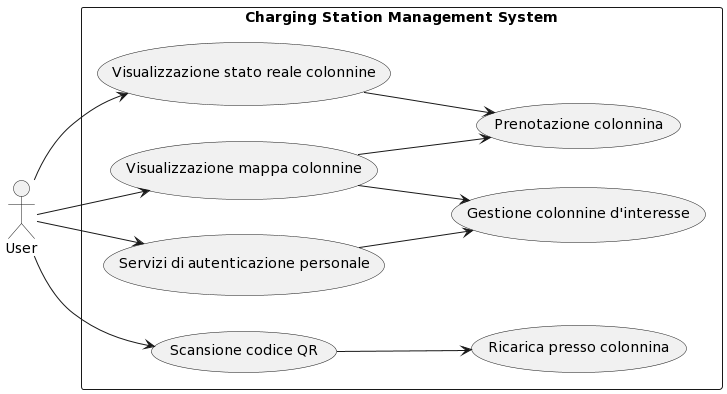
\includegraphics[width=\textwidth]{../images/casiduso.png}
    \caption{Diagramma dei Casi d'Uso}
    \label{fig:casiduso}
\end{figure}

\subsection{Requisiti Funzionali}
I requisiti funzionali descrivono le funzionalità specifiche che il sistema deve fornire,
come il sistema deve reagire a determinati input e come deve comportarsi in situazioni specifiche.\\


\begin{enumerate}[label=\arabic*.]
    \item Registrazione Utente
          \begin{enumerate}[label=\arabic{enumi}.\arabic*]
              \item Gli utenti devono poter creare un account fornendo informazioni personali, tra cui nome, cognome, indirizzo email e password.
              \item L'applicazione deve verificare l'unicità dell'indirizzo email.
          \end{enumerate}

    \item Login Utente
          \begin{enumerate}[label=\arabic{enumi}.\arabic*]
              \item Gli utenti registrati devono poter effettuare il login inserendo l'indirizzo email e la password.
          \end{enumerate}

    \item Visualizzazione della Mappa delle Stazioni di Ricarica
          \begin{enumerate}[label=\arabic{enumi}.\arabic*]
              \item Gli utenti devono poter visualizzare la loro posizione all'interno di una mappa, dopo aver acconsentito all'utilizzo di geolocalizzazione.
              \item Gli utenti devono poter visualizzare una mappa interattiva che mostra la posizione delle stazioni di ricarica per veicoli elettrici all'interno del territorio limitrofo.
              \item Le stazioni devono essere rappresentate da icone distintive sulla mappa.
          \end{enumerate}

    \item Visualizzazione dello Stato delle Stazioni
          \begin{enumerate}[label=\arabic{enumi}.\arabic*]
              \item Gli utenti devono poter vedere lo stato di ciascuna stazione di ricarica direttamente sulla mappa. Lo stato può essere "occupata," "libera," o "in fase di ricarica."
              \item Cliccando su una stazione, gli utenti possono ottenere informazioni dettagliate sulla colonnina, incluso l'indirizzo.
          \end{enumerate}

    \item Prenotazione di una Stazione di Ricarica
          \begin{enumerate}[label=\arabic{enumi}.\arabic*]
              \item Gli utenti devono poter prenotare una stazione di ricarica disponibile tramite l'applicazione.
          \end{enumerate}

    \item Sblocco di una Stazione con QR Code
          \begin{enumerate}[label=\arabic{enumi}.\arabic*]
              \item Gli utenti devono poter sbloccare una stazione di ricarica prenotata o libera utilizzando un codice QR posizionato sulla colonnina.
              \item L'applicazione deve poter leggere il codice QR, dopo la richiesta di utilizzo della fotocamera del dispositivo.
          \end{enumerate}

    \item Gestione delle Stazioni d'Interesse
          \begin{enumerate}[label=\arabic{enumi}.\arabic*]
              \item Gli utenti possono aggiungere stazioni di ricarica alla loro lista di "stazioni d'interesse."
              \item Devono poter rimuovere stazioni dalla lista d'interesse in qualsiasi momento.
          \end{enumerate}

    \item Localizzazione
          \begin{enumerate}[label=\arabic{enumi}.\arabic*]
              \item L'applicazione deve supportare servizi di geolocalizzazione in tempo reale.
          \end{enumerate}
\end{enumerate}

\subsection{Requisiti non Funzionali}
I requisiti non funzionali sono criteri e specifiche che definiscono il comportamento complessivo di un sistema software o di un'applicazione, ma non si concentrano direttamente sulle funzionalità principali.

Nel caso di \textit{Smart Charging Stations}:

\begin{enumerate}[label=\arabic*.]
    \item Performance: L'applicazione deve essere altamente performante, consentendo agli utenti di accedere rapidamente alle informazioni sulle stazioni di ricarica e di effettuare prenotazioni senza ritardi significativi.

    \item Usabilità: L'interfaccia utente dell'applicazione deve essere intuitiva e user-friendly, garantendo un'esperienza d'uso piacevole. In particolare, le mappe devono essere facili da navigare, e le operazioni di prenotazione e sblocco delle stazioni devono essere semplici da eseguire.

    \item Disponibilità: Il sistema deve essere disponibile 24/7, in modo che gli utenti possano accedervi in qualsiasi momento per visualizzare le stazioni di ricarica e effettuare prenotazioni.

    \item Compatibilità: L'applicazione deve essere compatibile con una vasta gamma di dispositivi mobili, inclusi smartphone e tablet, e deve funzionare su diverse piattaforme, come iOS e Android.

    \item Scalabilità: Il sistema deve essere progettato per gestire un grande numero di utenti simultanei senza degradazione delle prestazioni.

    \item Manutenzione e Aggiornamenti: Il sistema deve essere facilmente manutenibile e consentire l'aggiornamento regolare per introdurre nuove funzionalità e correzioni di bug.
\end{enumerate}

\subsection{Requisiti di Implementazione}
I requisiti di implementazione sono specifici per il sistema software e definiscono le caratteristiche tecniche che il sistema deve soddisfare.

\begin{enumerate}[label=\arabic*.]
    \item Linguaggio di programmazione: L'applicazione deve essere sviluppata utilizzando il linguaggio di programmazione Scala lato server per gestione delle colonnine, deve utilizzare il framework Express.js lato web server e il linguaggio Svelte per quanto riguarda l'interfaccia utente.
    \item Architettura Orientata agli Attori con Akka HTTP: L'implementazione deve aderire al paradigma basato su attori, sfruttando il framework Akka, incluso Akka HTTP, per gestire l'interazione tra i nodi del sistema.
    \item Tecnologie di Persistenza: La componente responsabile della conservazione dei dati deve essere sviluppata utilizzando MongoDB ed interfacciarsi con il server Node.
\end{enumerate}



% ===============================
% In questa sezione esporre brevemente i requisiti a cui il sistema proposto deve rispondere, concentrando l'attenzione sugli aspetti più rilevanti e facendo eventualmente uso di opportuni diagrammi di alto livello.\\

% Vincoli circa la lunghezza della sezione (escluse didascalie, tabelle, testo nelle immagini, schemi):

% \vspace{1cm}
% \begin{tabular}{l|rr}
%                  & Numero minimo di battute & Numero massimo di battute \\
%     \hline
%     1 componente & 4000                     & 6000                      \\
%     2 componenti & 6000                     & 8000                      \\
%     3 componenti & 8000                     & 10000                     \\
%     \hline
% \end{tabular}


\newpage
